\documentclass[a4paper]{article}

\usepackage[french]{babel}
\usepackage[utf8]{inputenc}
\usepackage[T1]{fontenc}
\usepackage{listings}
\usepackage{graphicx}
\usepackage[left=2cm,right=2cm,top=2cm,bottom=2cm]{geometry}

\lstset{
	numbers=left
}

%%%%%%%%%%%%%%%%  TIPS - LATEX  %%%%%%%%%%%%%%%%%%%%%%%
% ° Afficher une photo:
%   - Toutes photos doivent etre dans le dossier src
%   - Tu peux modifier la taille (scale)
%
%\begin{figure}[!h]
%	\centering
%	\includegraphics[scale=0.8]{src/NOM_DU_FICHIER.png}
%	\caption{LEGENDE DE LA PHOTO (OBLIGATOIRE) }
%\end{figure}
%
%======================================================
%
% ° Faire un encadré:
%
% \fbox{
%	CONTENU ENCADRE
% }\\
%
%========================================================
% ° Inclure un code source/programme:
%	- Les parametres firstline et lastline ne sont pas obligatoire
%
% \fbox{
%	\lstinputlisting[language=Python,firstline=3, lastline=10]{../Bloc.py}
% }\\
%
%%%%%%%%%%%%%%%%%%%%%%%%%%%%%%%%%%%%%%%%%%%%%%%%%%%%%%%%%%%



\begin{document}
    %%%%%%%%%%%%%%%%%%%%%%%%%%%%%%%%%%%%%%%%%%
\begin{titlepage}
	\centering
    \vspace*{0.5 cm} 
    \textsc{\LARGE Projet - Grammaires et langages}\\[1.0 cm]
    \textsc{\large Transformation et minimisation d'automate}\\[1.0 cm]
	\rule{\linewidth}{0.2 mm} \\[0.4 cm]
	
\includegraphics[scale=1]{src/logo.png}\\
	\vspace{0.5cm}
	\textsc{\Large Faculté des Sciences et Techniques}\\[0.2 cm]
	\textsc{\large Licence 3 Informatique }\\
	\rule{\linewidth}{0.2 mm} \\[1.5 cm]
	\begin{minipage}{0.4\textwidth}
	\begin{flushright} \large
		\emph{Encadré par :}\\
		Pr Philippe GABORIT\\
		\end{flushright}
    	\begin{flushright} \large
		\emph{Réalisé par :}\\
		Jérémy DRON \\
		\end{flushright}
	\end{minipage}\\[2 cm]
\end{titlepage}

%%%%%%%%%%%%%%%%%%%%%%%%%%%%
\section{Algorithme de transformation d'un AFN en AFD}

En théorie des automates, il existe plusieurs types d'automates ayant des 
caractèristique bien défini:\\

\begin{itemize}
	\item \textbf{AFD [Automate Fini Déterministe]:} Une seule transition au plus pour 
	chaques symboles depuis un état
	\item \textbf{AFN [Automate Fini Non-déterministe]:} Automate pouvant posséder plusieurs
 transitions pour chaques symboles depuis un état
 	\item \textbf{AFN-$\epsilon$ [Automate Fini Non-Déterministe avec $\epsilon$ transition]:} Automate possédant des transitions
 	avec le symbole du vide\\
\end{itemize}

Il est possible de passer d'un type d'automate à un autre en lui appliquant quelques modifications. Pour
passer d'un AFN à un AFD, il faut créer des super-états qui seront la combinaisons de plusieurs états.
Un état sera final si un des états qui le compose l'est. Mon algorithme ne 
prendra en entrée que les automates suivant: \\

A=\{Q,$\epsilon$,$\delta$,$q_0$,F\}\\
Q => L'ensembles des états de l'automate avec $|Q|<=10$\\
$\epsilon$ => L'alphabet de symbole fini avec $\epsilon={a,b}$\\
$\delta$ => Transitions de l'automate\\
$q_0$ => L'etat initial de l'automate\\
F => L'ensemble des états finaux\\
\subsection{Représentation d'un automate et structure de données}

Dans un premier temps, il a fallu pouvoir représenter un automate de manière que mon
programme puisse le comprendre et l'utiliser. Pour cela, j'ai réalisé pour
chaques symboles une matrice. Ces matrices continennent uniquement des "0" ou des "1"
et chaques lignes indiquent l'état de départ d'une transition et chaque colonne l'état 
d'arrivé.\\

\begin{center}
   \begin{tabular}{| l ||*{4}{c|} }
     \hline
       & 0 & 1 & 2 & 3 \\ \hline\hline
     0 & 1 & 1 & 0 & 0 \\ \hline
     1 & 0 & 0 & 1 & 0 \\ \hline
     2 & 0 & 0 & 0 & 0 \\ \hline
     3 & 0 & 0 & 0 & 0 \\
     \hline
   \end{tabular}
 \end{center}
Le tableau ci-dessus représente un matrice concernant un symbole d'un automate.\\

Pour réaliser un programme qui transforme un AFN en AFD, j'ai conçu le diagramme de 
classe suivant.\\

\begin{figure}[!h]
	\centering
	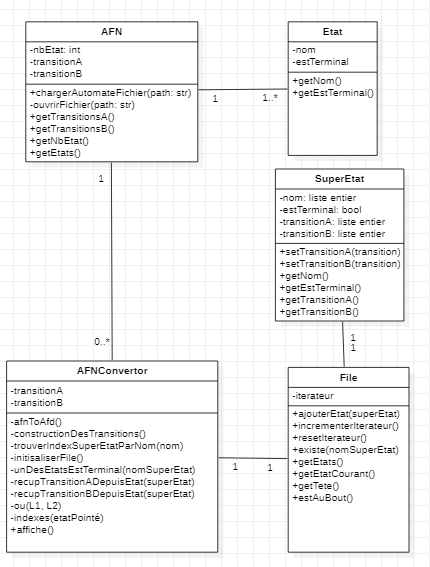
\includegraphics[scale=0.8]{src/diagramme_afnToAfd.PNG}
	\caption{Diagramme du programme de conversion d'AFN en AFD}
\end{figure}

\newpage
\subsection{Principe de l'algorithme}

Avant de programme l'algorithme, j'ai essayé de réaliser de manière manuscrit une transformation
d'un AFN et AFD en faisant uniquement des opérations qui pourraient être simple pour un programme.\\

De cette étape sur feuille, j'ai alors séparé mon programme en trois étapes. La première consiste
à initialiser le programme de transformation. La deuxieme étape consiste à creer des super états et
leurs transitions. Finalement, la dernière étape est la transformation des transitions trouver en 
transition utilisant les super-états. En effet, la deuxieme étape permet de trouver les transitions
des super-états qui utilise les états présent. Il faut alors indiquer à ces super-états qu'ils
faut qu'ils s'utilisent eux-même.\\

\begin{figure}[!h]
	\centering
	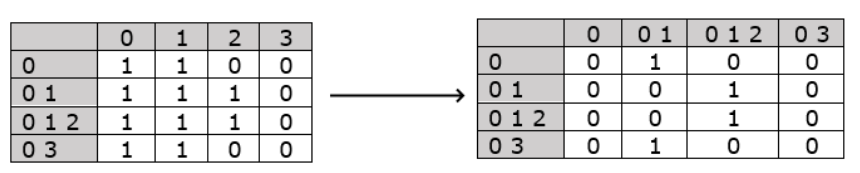
\includegraphics[scale=0.6]{src/etape3_AFNtoAFD.PNG}
	\caption{Transformation des transitions en utilisant les nouveaux super-états}
\end{figure}

En premier lieu, l'utilisateur va devoir charger une \textit{AFN} dans le programme puis
renseigner un chemin vers un fichier où est inscris les informations de l'automate. Par la 
suite, il faut utiliser un objet de type \textit{AFNConvertor} qui va convertir l'automate.
Finalement, pour l'afficher l'utilisateur doit afficher le convertisseur. 

Pour charger dans notre programme l'automate, le programme prend en entréer un fichier texte
qui contient toutes les informations sur l'automate. Sur la première ligne est inscris le 
nombre d'états de l'automate, sur la deuxième ligne les états terminaux puis sur les lignes
suivantes les matrices de transitions de chaques lettres de l'alphabet. Voici un exemple, ci-après:\\

\fbox{
	\lstinputlisting[]{../AFNtoAFD/automate.txt}
}\\

Par ailleurs, c'est le constructeur de l'objet convertisseur qui va lancer la conversion.
L'avantage est que l'utilisateur ne peut pas afficher l'\textit{AFD} avant de le convertir. La 
conversion est ordonnée par la methode \textit{afnToAfd()} qui reprend les trois étapes 
de l'algorithme ci-dessus.\\

\fbox{
	\lstinputlisting[language=Python,firstline=14, lastline=24]{../AFNtoAFD/AFNconvertor.py}
}\\

La première étape, permet d'initialiser une file. Cette file prend initialement l'état 
initial de l'automate que j'ai concidéré comme l'état "0" de l'automate. Le super-état initial
contient un nom et des transitions pour chaques lettres de l'alphabet. Cette file va 
permettre d'arrêter le processus de recherche lorsque le programme l'aura parcourus 
entierement.\\

La deuxième étape, commence par recuperer les transitions de 
l'état courant de la file qui se présente en une liste de "0" ou/et "1".
Ces listes permettent de recuperer la composition des super-états qu'elles vont
générer. Dans notre cas la composition est lié au nom. Par la suite, le programme va 
chercher à savoir si le super-états en cours de construction est terminal ou non, cela
grâce à la méthode \textit{unDesEtatsEstTerminal()}.\\

\fbox{
	\lstinputlisting[language=Python,firstline=104, lastline=116]{../AFNtoAFD/AFNconvertor.py}
}\\

Pour finir cette étape de l'algorithme, lorsque le programme à toutes les informations pour générer le.s super-état.s il 
verifie s'il existe dans la file. Si le.s super-état.s existe.nt déjà alors il modifie les 
transitions de ce.s dernier.s sinon il le.s crée dans la file.\\ 

Dans la dernière partie de l'algorithme, le programme va transformer les transitions en utilisant
les nouveaux super-états. Le programme va concidérer deux matrices, pour chaques lettres
de l'alphabet. Le programme va remplir la matrice en utilisant la position des super-états
dans la file. Ainsi, le super-états en position "2" de la file sera représenté en ligne
(état de départ) en position "2" et également représenté en colonne (état d'arrivé) en 
position "2". Pour récuperer la position du super-état dans la file le programme fait une
recherche par son nom qui est unique, grâce à la methode \textit{trouverIndexSuperEtatParNom()}.\\

\fbox{
	\lstinputlisting[language=Python,firstline=43, lastline=55]{../AFNtoAFD/AFNconvertor.py}
}\\

Par ailleurs, j'ai fais le choix d'afficher l'AFD à la fin du programme et non de générer un AFD pour un programme car
la représentation que je fais des automates ne me permet pas de préciser le nom des états. J'aurais
donc perdu de l'informations utile à l'exercice. Toutefois, cela est possible en apportant quelques 
modifications.\\


\subsection{Programme et execution}

	Pour montrer le fonctionnement de mon programme nous concidérons l'automate suivant:

\begin{figure}[!h]
	\centering
	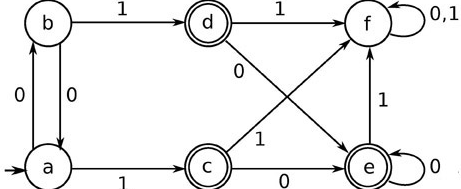
\includegraphics[scale=0.4]{src/auto2.png}
	\caption{Automate d'état fini non déterministe}
\end{figure}

Le caractère non déterministe de cette automate est visible depuis l'état initial qui possède
deux transitions de "a".

La représentation de notre automate pour le programme sera la suivante :\\

\fbox{
	\lstinputlisting{../AFNtoAFD/automate.txt}
}\\

Lors de l'execution, le programme à bien charger notre automate en mémoire.
\begin{figure}[!h]
	\centering
	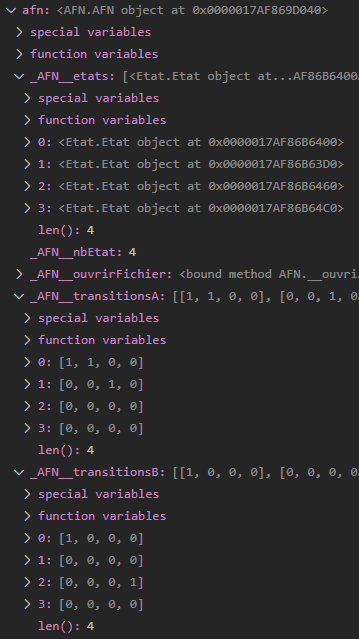
\includegraphics[scale=0.8]{src/AfnCharge.PNG}
	\caption{Automate du fichier chargé en mémoire}
\end{figure}
\newpage

Une fois l'automate chargé en mémoire il est passé au convertisseur qui
va chercher les super-états puis les sauver en file.\\

\begin{figure}[!h]
	\centering
	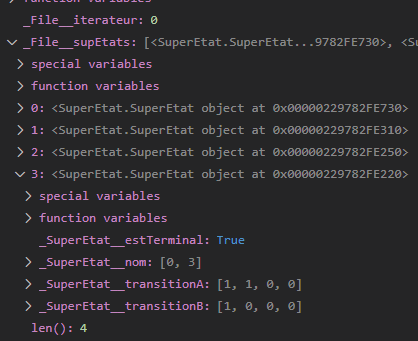
\includegraphics[scale=0.7]{src/AFNfile.PNG}
	\caption{File contenant les super-états à la fin du processus de recherche}
\end{figure}

Il est possible de voir qu'il a trouvé quatre super-états dont un qui 
concidère comme terminal. Cela semble correcte car ce super-état est 
composé des états "0" et "3" or "3" est terminal. Par ailleurs, il est possible 
de remarquer que les transitions ne n'ont pas encore pris en compte les nouveaux
état puisqu'elles continennent plusieurs "1".

Il est possible d'observer la dernière étape de l'algorithme (prise en compte des nouveaux
états par les transitions) soit dans la console de déboggage ou direct en observant le résultat
en console.\\

\begin{figure}[!h]
	\centering
	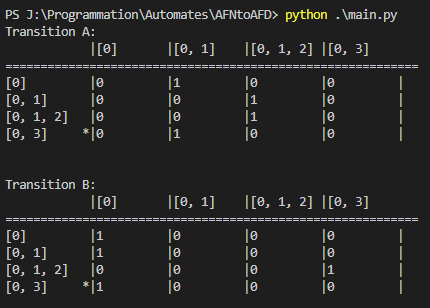
\includegraphics[scale=0.8]{src/resultat_AFN.PNG}
	\caption{Resultat de la conversion de l'AFN en AFD}
\end{figure}

Il est possible de voir un "*" sur une entête d'une ligne des transitions, cela correspond
à l'état terminal. Nous pouvons constater que les matrices de transitions continennent uniquement
un seul et unique "1" sur chaque ligne, l'automate est alors déterministe.

Par ailleurs, le résultat du programme correspond au nouvel automate que j'avais trouvé préalablement.

\newpage

\section{Algorithme de minimisation d'un automate}

A présent, je cherche à minimiser un AFD, cest-à-dire que je
cherche à avoir un automate avec le minimum d'état qui a le même
comportement que celui actuel. En effet, certains automates ont
des états qui peuvent être combiner entre-eux. Mon algorithme ne 
prendra en entrée que les automates suivant: \\

A=\{Q,$\epsilon$,$\delta$,$q_0$,F\}\\
Q => L'ensembles des états de l'automate avec $|Q|<=10$\\
$\epsilon$ => L'alphabet de symbole fini avec $\epsilon={a,b}$\\
$\delta$ => Transitions de l'automate\\
$q_0$ => L'etat initial de l'automate\\
F => L'etat final de l'automate\\



\subsection{Représentation d'un automate et structure de données}

Premièrement, j'ai cherché une représentation, pour mon
AFD, que mon programme pourrait facilement utiliser. Nous 
nous sommes alors basés de ce que j'avais trouvé dans la 
première partie.\\
J'ai pour chaque symbole de l'alphabet une matrice lui correspondant. Dans
le cas précédent la matrice contenait l'information de quels états
de départ pointaient sur quels états d'arrivés. Dans le cas présent,
c'est l'inverse, je cherche à savoir quels états est pointés par
quels états. Dû au fait, que je travaille uniquement avec des AFDs
j'ai pu concidérer que:\\

Soit M = "La matrice des transitions de départ vers arrivé"
alors $M^t$ = "La matrice des transitions des arrivés vers les départs"\\

Par ailleurs, pour minimiser l'automate j'ai utilisé l'algorithme vu
en cours. Dans mon programme, j'utilise une file qui contiendra les
couples d'états à vérifier. J'ai fait le choix de faire mon programme
dans le paradygme orienté objet pour une optimisation de la compléxité cognitive.
J'ai réalisé le diagramme de classe du programme pour faciliter
la compréhension de la structure du programme.

\begin{figure}[!h]
	\centering
	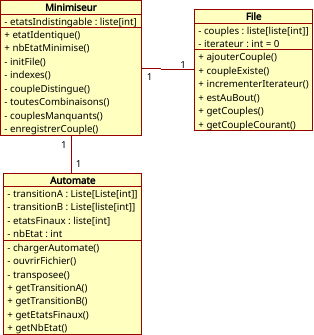
\includegraphics[scale=0.8]{src/diagramme_minimiseur.png}
	\caption{Diagramme de classe du minimiseur d'automate}
\end{figure}


\subsection{Principe de l'algorithme}

En premier lieu, l'utilisateur doit créer un objet de type \textit{Automate} et 
un objet de type \textit{Minimiseur} puis il peut utiliser deux méthodes:
une permettant de récuperer les états non distingables et l'autre le nombre
d'état de l'automate minimisé.\\

\fbox{
	\lstinputlisting[]{../Minimisation/main.py}
}\\

Concretement, l'objet \textit{Automate} prend un fichier en entrée qui contient des informations sur
l'automate ainsi la représentation de l'automate exprimé plus haut. Le fichier 
doit contenir sur la premier ligne le nombre d'état de l'automate, sur la deuxieme
ligne les états terminaux et finalement les matrices de transitions sur les lignes suivantes.
Le fichier peut ressembler à ça:\\

\fbox{
	\lstinputlisting[]{../Minimisation/automate.txt}
}\\

C'est grâce à ce fichier que l'automate peut être charger dans le programme, donc le respect
de la forme est essentiel pour le fonctionnement.\\

Pour minimiser l'automate, le \textit{minimiseur} va initialiser la file avec les distingués
trivialement, i.e. les terminaux et non terminaux. Par la suite, le programme va générer de
nouveaux couples d'états distingués qu'il va ajouter en file si ces derniers n'existent pas
déjà. Le programme va parcourir toute la file jusqu'à arriver en tête avant de récuperer les
états des couples manquants. Pour connaitre le nombre d'état de l'automate final, le \textit{minimiseur}
soustrait au nombre d'état actuel le nombre d'état non distingué.\\

Pour trouver les états distingués engendré par un couple d'état passé en entrée de la fonction,
le programme vient recupérer grâce
à la matrice les états pour lesquels il y a une transition avant d'enregistrer dans la file toutes
les combinaisons d'états non existantes. Si un état d'entrée engendre aucun état de sortie, càd
si un état ne possède pas de transition pour un symbole de l'alphabet, alors
le programme ignore les transitions de ce symbole pour cet état.

\fbox{
	\lstinputlisting[language=Python,firstline=43, lastline=73]{../Minimisation/Minimiseur.py}
}\\

Pour récuperer les couples manquants, le programme génère tous les couples possibles puis
il supprime un par un tous ceux qui existe dans la file. Les couples qui restes sont ceux
qui n'existent pas en file donc ceux indistingables. Le programme vient effectuer l'opération
ensembliste suivantes:\\

	soit:\\
	$A=$\{Ensemble des couples d'états distingués que possède la file\}\\
	$\bar{A}=$\{Ensemble des couples d'états indistingués\}\\
	$\Omega=$\{Ensemble des couples d'états possibles\}\\

	Je cherche à avoir $\bar{A}$.\\

	$\bar{A}=\Omega-A$

Pour récuperer les états indistingables, il a suffit de prendre les états existant au moins
une fois dans les couples de $\bar{A}$.

\subsection{Programme et execution}

Dans cette partie, je vais détailler quelques méthodes du programme permettant le bon
fonctionnement de l'algorithme décrit ci-avant puis je vais le mettre en pratique avec un exemple.\\

Le programme tient essentiellement sur des matrices contenant des transitions d'état. Pour pouvoir
récuperer depuis un état les états qui pointent vers lui nous avons développé la methode 
\textit{indexes()}. Cette méthode recupère les numéros des colonnes de la matrice pour une ligne donnée.

\fbox{
	\lstinputlisting[language=Python,firstline=75, lastline=89]{../Minimisation/Minimiseur.py}
}\\

Avant de pouvoir ajouter en file tous les états distingués engendré par un couple d'état, il faut
pouvoir trouver toutes les combinaisons de couples d'états. Pour cela la méthode \textit{toutesCombinaisons()}
permet d'associer les états entre-eux.\\

\fbox{
	\lstinputlisting[language=Python,firstline=91, lastline=102]{../Minimisation/Minimiseur.py}
}\\

Cette méthode se contente uniquement de faire toutes les combinaisons possibles, c'est la méthode appelante
qui va gérer les doublons par exemple.\\

\textbf{\underline{Exemple:\\ }}

Concidérons l'automate suivant:\\


\begin{figure}[!h]
	\centering
	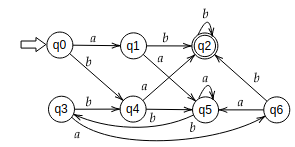
\includegraphics[scale=0.8]{src/auto1.png}
	\caption{Automate du premier exemple}
\end{figure}

La représentation de l'automate pour le programme sera la suivante:\\

\fbox{
	\lstinputlisting[]{../Minimisation/automate.txt}
}\\

Grace au fichier l'automate est chargé correctement dans le programme.\\

\begin{figure}[!h]
	\centering
	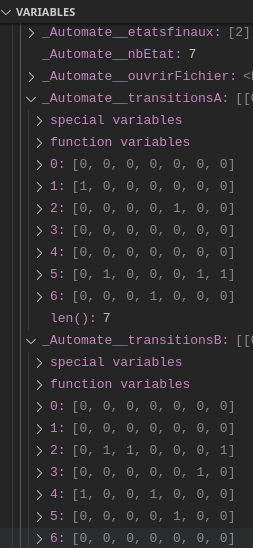
\includegraphics[scale=0.4]{src/autoCharge.png}
	\caption{Automate chargé en mémoire du programme}
\end{figure}

Nous pouvons constater que toutes les informations sont chargées en mémoire
et les transitions sont les transposées des matrices du fichier. Par ailleurs, 
nous pouvons observer la file durant l'execution et voir qu'elle contient
les couples de l'initialisation et ceux trouvés lors du déroulement

\begin{figure}[!h]
	\centering
	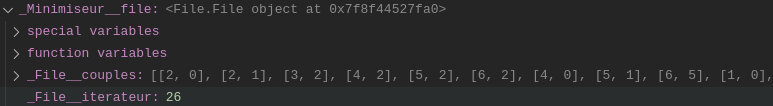
\includegraphics[scale=0.5]{src/fileExecution.png}
	\caption{Une partie de la file à la fin de l'execution}
\end{figure}

Après execution du programme, j'obtiens la sortie suivante qui correspond à ce
que j'ai trouvé lors de mes recherches manuel en amont.

\begin{figure}[!h]
	\centering
	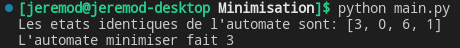
\includegraphics[scale=0.5]{src/resultat_auto1.png}
	\caption{Affichage du programme pour l'automate de l'exemple}
\end{figure}


\end{document}
